\documentclass[a4paper, titlepage]{jsarticle}

\date{\today}
\usepackage[dvipdfmx]{graphicx}
\usepackage{url}
\usepackage[T1]{fontenc}
\usepackage{float}
\usepackage{ascmac}

\title{ドローン宅配事業者支援システム}

\author{土佐山田IT株式会社}

\begin{document}
\maketitle

\tableofcontents

\clearpage

\section{現状の課題}

\section{課題の解決方法}

\section{機能の概要・前提条件・制約事項}

\section{情報・金銭の流れ}

\subsection{情報の流れ}
本システムにおける情報の流れを図\ref{fig:info_flow_1}に示す.
本システムは,利用者(送り主及び受け取り主)が使用する端末,宅配事業者が利用する端末,システム管理者が利用する端末及び,システム中核を担うサーバとデータベースによって構成される.

各ユーザからの要求を受けサーバが処理を行い,webページやアプリケーションに適した情報を提供する.

\begin{figure}[H]
  \centering
  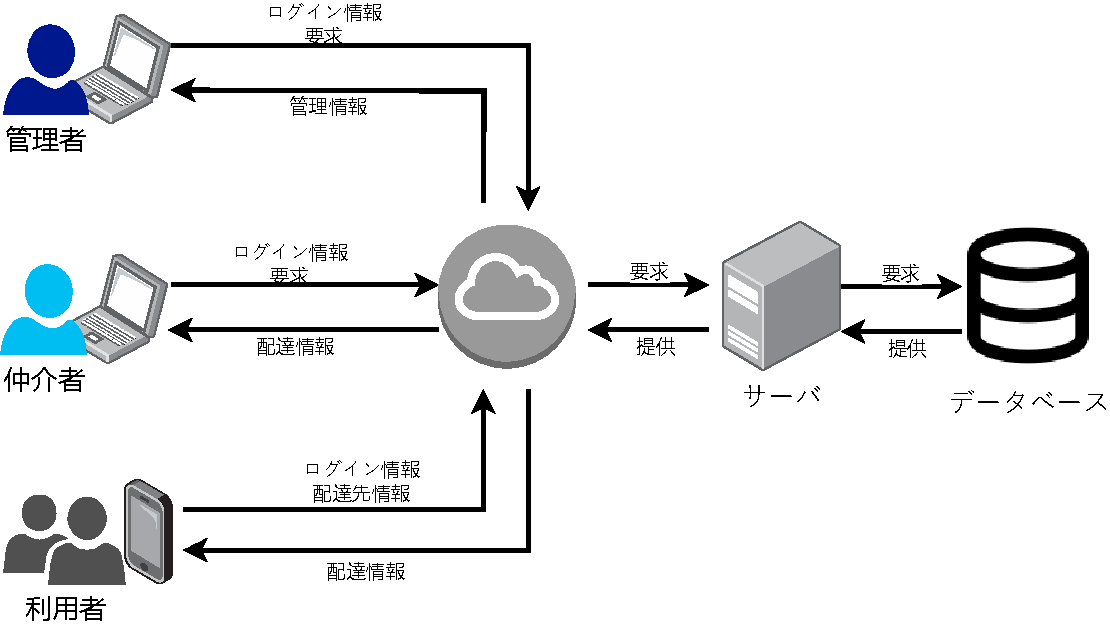
\includegraphics[width=0.6\linewith]{./info_flow.pdf}
  \caption{本システムにおける情報の流れ}
  \label{fig:info_flow_1}
\end{figure}

\subsection{金銭の流れ}
本システムにおける金銭の流れを図\ref{fig:money_flow_1}に示す.

\begin{figure}[H]
  \centering
  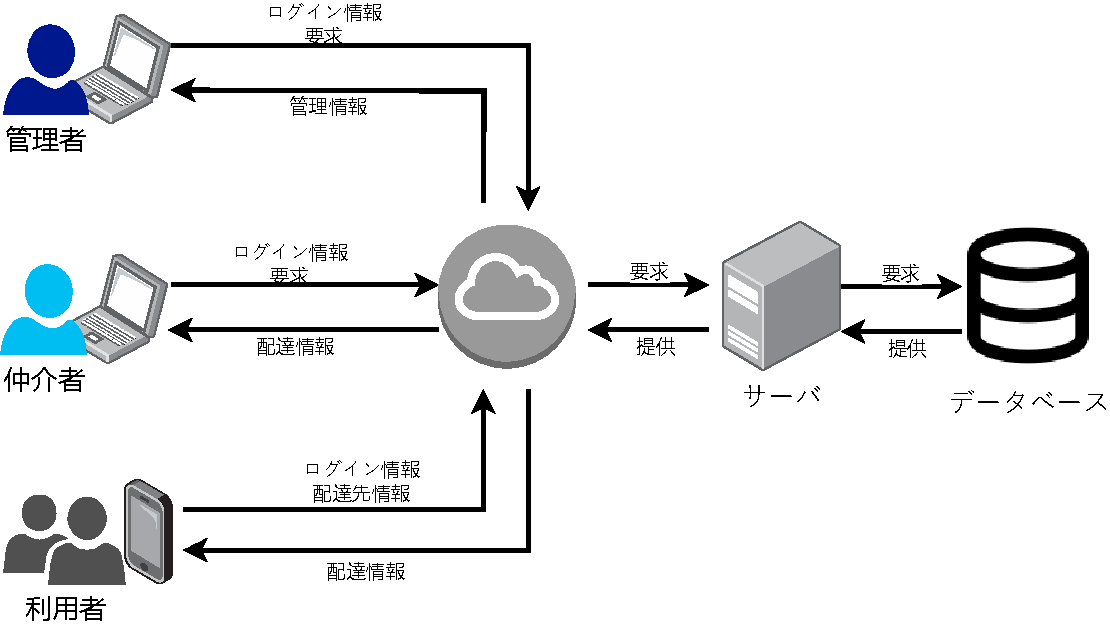
\includegraphics[width=0.6\linewith]{./info_flow.pdf}
  \caption{本システムにおける金銭の流れ}
  \label{fig:info_flow_1}
\end{figure}


\section{想定する利用者}

\section{運用・保守}

\section{ハードウェア・ソフトウェアの構成}

\section{費用・効果}

\section{スケジュール}

\section{本システムのアピールポイント}

\section{貢献度}


\end{document}
